\documentclass[12pt, letter]{article}

%% Class name and Assignment number
%%
\newcommand{\courseName}{Introduction~to~Deep~Learning~for~Computer~Vision}
\newcommand{\assignName}{Assignment~3:~Simple~Linear~Classifier II}

%% Packages
\usepackage{amsmath,amsfonts,amssymb,amsthm,dsfont}
\usepackage{graphicx}
\usepackage[bookmarks=false]{hyperref}
\usepackage{color}
\usepackage{lipsum}

%% Paper format
\usepackage{geometry}
\geometry{
    letterpaper,
    %% total={216mm,279mm}, %< NSERC size
    margin=2.00cm,     %< default
    %% margin=1.87cm,       %< NSERC tightest
}

%% Headers and footers
\usepackage[explicit]{titlesec}
\newpagestyle{titlesec_assignment}{
  \sethead{\courseName}{}{\assignName}\setfoot{}{\thepage}{}
  \headrule
  %% \footrule
}

\begin{document}

%% Set header and footer
\pagestyle{titlesec_assignment}

%% Title
\title{\courseName\\\assignName}
\author{Paul Molina-Plant}
\maketitle

\abstract{TODO}

\pagebreak

\section{Derivation of the gradient for cross entropy}
The cross entropy function.
\begin{equation}
  L_{i} = - log \frac{\sum_{j}t_{ij}e^{s_{ij}}}{\sum_{j}e^{s_{ik}}}
\end{equation}
I assume log base e for (1).
\begin{equation}
  P_{ij} = \frac{e^{s_{ij}}}{\sum_{k}e^{s_{ik}}}
\end{equation}
\begin{equation}
  t_{ij} =
  \begin{cases}
    1 & j = y_{i} \\
    0 & j \ne y_{i}
  \end{cases}
\end{equation}
Simplifying (1) by replacing softmax with (2) and reducing the sum following (3).
\begin{equation}
  L_{i} = - ln \frac{\sum_{j}t_{ij}e^{s_{ij}}}{\sum_{j}e^{s_{ij}}} = - ln \sum_{j}t_{ij}P_{ij} = - ln P_{ij}
\end{equation}
Computing the partial derivative of (2) with respect to $s_{j}$.
\begin{equation}
  i = j \longrightarrow \frac{\partial P_{ij}}{\partial s_{j}} =
  \frac{e^{s_{ij}} \sum_{k}e^{s_{ik}} - e^{s_{ij}}e^{s_{ik}}}{(\sum_{k}e^{s_{ik}})^2} =
  \frac{e^{s_{ij}}}{\sum_ke^{s_{ik}}} \left(\frac{\sum_ke^{s_{ik}}e^{s_{ik}}}{\sum_ke^{s_{ik}}}\right) =
  P_{ij} (1  - P_{ik})
\end{equation}
\begin{equation}
  i \ne j \longrightarrow \frac{\partial P_{ij}}{\partial s_{j}} = \frac{- e^{s_{ij}}e^{s_{ik}}}{(\sum_{k}e^{s_{ik}})^2} = - \frac{e^{s_{ij}}}{\sum_ke^{s_{ik}}} \left(\frac{e^{s_{ik}}}{\sum_ke^{s_{ik}}}\right) = - P_{ij}P_{ik}
\end{equation}
\begin{equation}
  \delta_{ij} =
  \begin{cases}
    1 & i = j \\
    0 & i \ne j
  \end{cases}
\end{equation}
The partial derivaties (5) and (6) may be combined using (7).
\begin{equation}
  \frac{\partial P_{ij}}{\partial s_{j}} =
  \begin{cases}
    P_{ij}(1 - P_{ik}) & i = j \\
    - P_{ij}P_{ik} & i \ne j
  \end{cases}
   = P_{ij} (\delta_{ij}  - P_{ik})
\end{equation}
Computing the partial derivative of (4) with respect to $s_j$.
\begin{equation}
  \frac{\partial L_i}{\partial s_j} = - \frac{1}{P_{ij}} \frac{\partial P_{ij}}{\partial s_{j}} = \delta_{ij} - P_{ik}
\end{equation}
\begin{equation}
  s_{ij} = Wx_{ij} - b
\end{equation}
Computing the partial derivative of (8) with respect to $W$.
\begin{equation}
  \frac{\partial s_j}{\partial w} =
  \begin{cases}
    x_{ij} & i = j \\
    0 & i \ne j
  \end{cases}
\end{equation}
\begin{equation}
  i = j \longrightarrow \frac{\partial L_i}{\partial W} =
  \frac{\partial L_i}{\partial s_j} \frac{\partial s_j}{\partial W} =
  - \frac{x_{ij}e^{s_{ij}}\sum_ke^{s_ik} - e^{s_{ij}}x_{ik}e^{s_{ik}}}{(\sum_ke^{s_{ik}})^2} =
  - = - e^
\end{equation}

\pagebreak

Example Section.

\subsection{Example Subsection}

Example Sub Section.

\paragraph{Example paragraph.}


\subsection{Example  Equation}

This is how a equation looks like.
\begin{equation}
  y = a x^2 + b x + c
  \;\;,
\end{equation}
where an inline equation looks like $a=b$.

\subsection{Example  Figure}

To put a figure, you can do as shown in Fig.~\ref{fig:eg}.
%%
\begin{figure}
  \centering
  \rule{2cm}{2cm} % Replace this with below, and your actual figure
  %% 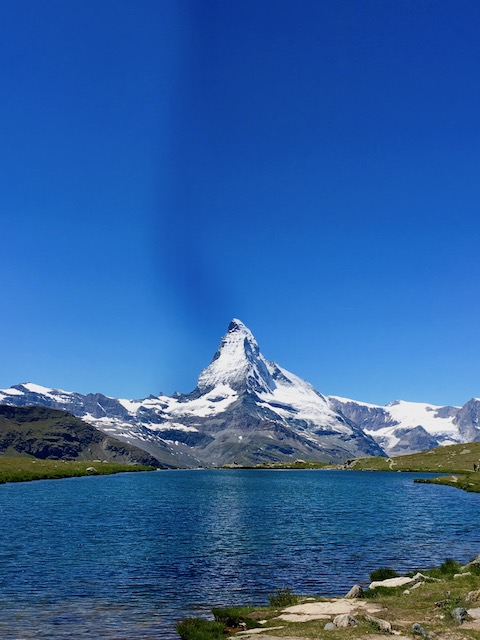
\includegraphics[width=0.4 \textwidth]{input.jpg}
  \caption{Example caption.}
  \label{fig:eg}
\end{figure}

\end{document}


%%% Local Variables:
%%% mode: latex
%%% TeX-master: t
%%% End:
